Este capítulo detalha o BFT-SMaRt apresentando seu conceito, princípios de Design, protocolos centrais, reconfiguração, implementação, configurações alternativas e finalizando nas conclusões do capítulo.


%	\section{BTF-SMART}
	\section{Conceitos}
	Na área da computação, a  replicação de máquina de estado (SMR), é um método para implementação de um serviço tolerante a falha em que um conjunto de servidores trabalham coordenadamente na interação com a máquina cliente e o serviço está implantado neste conjunto em vez de  apenas um. \\
	
	O BFT-SMART é uma biblioteca \textit{open-source} criado recentemente em linguagem Java que possui um conjunto de classes para implementar um sistema distribuído robusto consistindo de replicação de máquina de estado tolerantes a falhas bizantinas (falha bizantina ocorre quando uma máquina apresenta um comportamento arbitrário fora de sua especificação, por exemplo, quando um servidor é invadido e começa a rodar código malicioso) e apresentando confiabilidade, modularidade, reconhecimento de sistema multicore, suporte à reconfiguração e interface flexível de programação, como foi apresentado por Alchieri et al em \cite{bessani3}. \\
	
	Novamente em \cite{bessani3} é discutido como nos últimos anos a discurção sobre \textit{State Machine Replication (SMR)} tolerantes a falhas bizantinas (\textit{Byzantine Fault-Tolerant - BFT}) tem se acirrado contendo pouco avanço prático, apenas protótipos usados para validar ideias apresentadas em artigos, assim dificultando a aplicação dessa prática em aplicações reais. Os autores acreditam que isto seja devido à falta de implementações de um SMR BFT robusto. O BFT-SMaRt foi proposto tendo em mente contornar tal dificuldade, o qual almeja tanto alta performance em execuções livre de falhas quanto corretude mesmo com replicas que apresentam comportamento arbitrário. Incluindo o desenvolvimento de protocolos para transmissão de estados e reconfiguração. \\
	
	\section{Princípios do Design}
	
	%\begin{itemize}
		%\item Modelo Harmonioso de Falhas\\
		\subsection{Modelo Harmonioso de Falhas}
		BFT-SMaRt tolera falhas bizantinas não-maliciosas por padrão. Num modelo de sistema realistas mensagens podem ser enviadas, rejeitadas ou corrompidas, enquanto processos podem executar de forma anormal sem que ajam terceiros envolvidos. Além disso, também é possível configurar o BFT-SMaRt para que ele lide com falha bizantinas maliciosas, para tal ele provem assinaturas criptografadas. \\
		
		%\item Simplicidade\\
		\subsection{Simplicidade}
		A enfâse na corretude dos protocolos levou aos projetistas evitarem otimizações no código-fonte que poderiam acarretar em complexidade desnecessária tanto em tempo de desenvolvimento ou codificação. Este foi um dos motivos para a bibioteca ter sido desenvolvida em Java ou invés de outra slinguagends de programação em alto nível, como C/C++ ou Python.\\
		
		%\item Modularidade\\
		\subsection{Modularidade}
		BFT-SMaRt implementa um protocolo SMR modular que utiliza uma, bem definida, primitiva de consenso. Além de módulos responsáveis por garantir uma comunicação point-to-point confiável, ordenação de solicitações de clientes e o consenso entre SMRs, o BFT-SMaRt também implementa módulos de transferência de estados e reconfiguração, os quais são totalmente separados do protocolo de agreement.\\
		
		\begin{figure}[htb]
			\begin{center}
				
				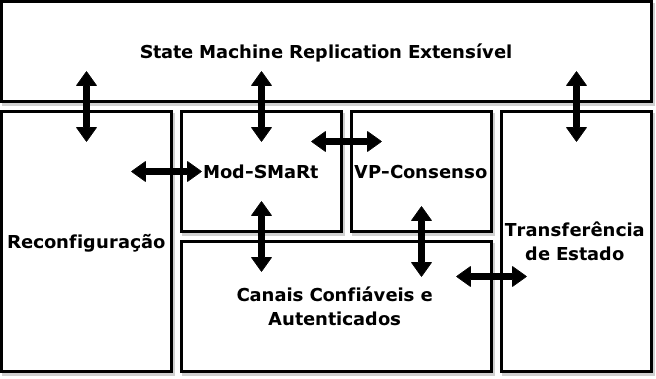
\includegraphics[clip,width=13.0cm]{images/image4.png}
				\caption{A modularidade do BFT-SMaRt. Adaptado de Alchieri~\cite{bessani3}}
				\label{fig:vis_sis}
			\end{center}
		\end{figure}
		
		%\item  Interface de Programação de Aplicação Simples e Extensível\\
		\subsection{Interface de Programação de Aplicação Simples e Extensível}
		A biblioteca java encapsula toda a complexidade do SMR BFT dentro de uma API que pode ser utilizada para a implementação de serviços determinísticos, utilizando métodos invoque(comando) para enviar comandos às réplicas quem implementam o método execute(comando) para que as réplicas processem o comando enviado. Entretanto, caso a aplicação necessite de comportamentos especializados não suportado por este modelo de programação, é possível utilizar outras chamadas ou plug-ins tanto no lado do cliente quanto do servidor.\\
		
		
		%\item Consciência de ambiente Multi-Core\\
		\subsection{Consciência de ambiente Multi-Core}
		BFT-SMaRt é capaz de aproveitar a arquitetura multicore dos servidores para diminuir o tempo de processamento em regiões críticas do protocolo.\\
		
		%\item Modelo do Sistema\\
		\subsection{Modelo do Sistema}
		BFT-SMaRt assume o modelo usual para sistemas BFT SMR: n $\geq$ 3f+1 réplicas para tolerar f falhas bizantinas. Entretanto, visto que o sistema suporta reconfiguração, é possível modificar n e f em tempo de execução. Além disso, o sistema permite ser configurado para utilizar apenas n $\geq$ 2f+1 réplicas para tolerar f falhas de sistema. Porém, independente da configuração, o sistema necessita de conexões point-to-point confiáveis entre os processos de comunicação. Essa conexão é realizada utilizando message authentication code (MAC) sobre o protocolo TCP/IP.\\
	%\end{itemize}
	
	\section{Protocolos Centrais}
	
	%\begin{itemize}
		%\item Total Order Multicast\\
		\subsection{Total Order Multicast}
		Em um sistema distribuído, um total order é um protocolo de mensagem broadcast que garante a entrega das mensagens de forma confiável e na mesma ordem para todos os participantes.\\
		
		Total Order Multicast é possível graças ao Mod-SMaRt, um protocolo modular que implementa BFT SMR utilizando uma primitiva de consenso. Durante sua fase de execução normal, a qual ocorre na ausência de falhas e na presença de sincronismo entre as outras réplicas, clientes enviam suas solicitações para todas as réplicas e aguardam pela resposta. Total order é alcançado através de uma sequência de instancias de consenso, cada uma delas decidindo sobre um lote de solicitações de clientes. Cada instância é composta por três passos de comunicação. O primeiro passo solicita que o líder do consenso envie uma mensagem de PROPOSE para cada réplica. Esta etapa é seguida por duas etapas de mensagens de todos para todos (all-to-all) compostas de mensagens WRITE e ACCEPT. Onde as mensagens de PROPOSE contém o lote de solicitações, WRITE e ACCEPT contém o hash criptografado de tal lote.\\
		
		Quando uma falha ocorre ou alguma replica encontra-se dessincronizada das demais, o Mod-SMaRt pode mudar de fase para a de sincronização. Durante esta fase um novo líder é eleito e as réplicas são forçadas a entrarem na mesma instância de consenso. Este “pulo” pode causar com que algumas réplicas ativem o protocolo de transferência de estados.\\
		
		%\item Transferência de Estado\\
		\subsection{Transferência de Estado}
		A fim de implementar uma SMR que possa ser usada na prática, faz-se necessário que as réplicas possam ser reparadas e reintegradas ao sistema sem que todo o sistema de replicação seja reiniciado. Para garantir tal característica, o BFT-SMaRt implementa algumas ideias chaves: (1) armazenar o log dos lotes de operações em execução em apenas um disco, (2) tirar snapshots em diferentes pontos da execução em várias réplicas e (3) realizar transferência de estados  de forma colaborativa, cada réplica enviando diferentes partes do estado para a réplica que está sendo recuperada.\\
	%\end{itemize}
	
	\section{Reconfiguração}
	BFT-SMaRt provem um protocolo especial que permite que réplicas sejam adicionadas ou executadas on-the-fly. Porém, tal processo só pode ser iniciado pelos administradores executando um cliente View Manager, por motivos de segurança.\\
	
	\section{Implementação}
	BFT-SMaRt foi desenvolvido contendo menos de treze mil e quinhentas linhas de código Java distribuídos em cerca de noventa arquivos. Tal característica é significativamente menor do que ocorre em sistemas similares que geralmente possuem mais de vinte mil linhas de código. \\
	
	Um ponto chave quando se está implementando um \textit{middleware} de replicação de alta vazão é como separar as várias tarefas do protocolo em uma arquitetura que seja eficiente e robusta. No caso de um \textit{Bizantine Fault Tolerante State Machine Replication} (BFT SMR) existem dois requisitos adicionais: o sistema precisa lidar com centenas de clientes e resistir a possíveis comportamentos maliciosos tanto dos clientes quantos das outras replicas.\\
	
	A Figura \ref{fig:image5} apresenta a arquitetura central com as \textit{threads}  usadas para o processamento das mensagens arquitetadas pela implementação do protocolo. Nesta arquitetura, todas as \textit{threads} comunicam através de filas delimitadas. A figura também mostra qual \textit{thread} alimenta e consume informações de cada fila. \\  
	
	\begin{figure}[htb]
		\begin{center}
			
			\includegraphics[clip,width=13.0cm]{images/image5.png}
			\caption{Processamento de mensagens arquitetadas entre replicas do BFT-SMaRt. Adaptado de Alchieri~\cite{bessani3} }
			\label{fig:image5}
		\end{center}
	\end{figure}
	
	As solicitações dos clientes são recebidas através da \textit{thread pool} provida pelo \textit{Netty Communitation Framework}. Assim que uma mensagem proveniente do cliente é recebida, é verificado se trata-se de uma solicitação ordenada ou não ordenada. Solicitações não ordenadas, as quais são geralmente aplicadas por comandos de apenas leitura, são entregadas diretamente para o serviço de implementação. No caso de uma solicitação ordenada, elas são entregues para o \textit{client manager}, o qual verifica a integridade da solicitação, caso esteja integra, a solicitação é encaminhada para a fila do respectivo cliente. Perceba que o endereço MAC dos clientes são verificados pelo \textit{Netty threads}, desta forma as maquinas multi-core e multi-processadas vão naturalmente aproveitar de seu poder para conquistar uma alta vazão. \\ 
	
	O \textit{proposer thread} é responsável por juntar um \textit{batch} de solicitações e transmitir a mensagem \textit{PROPOSE} do protocolo de consenso. O BFT-SMaRt preenche o \textit{batch} com solicitações pendentes até que: (a) seu tamanho alcance o máximo definido no arquivo de configuração; ou (b) não haja mais solicitações sobrando para serem adicionadas. Esta \textit{thread} só está ativa na replica líder. \\
	
	Cada mensagem \textit{m} que deve ser enviada de uma replica para outra é colocada na fila de saída (\textit{out queue}) pela qual uma \textit{sender thread} vai serializar a mensagem \textit{m}, produzir o endereço MAC que será anexado na mensagem e, enfim, enviar utilizando \textit{sockets TCP}. Do ponto de vista da replica que irá receber a mensagem, uma \textit{receiver thread} vai ler \textit{m}, autenticar (validar seu MAC), deserializar e colocar na fila de entrada (\textit{in queue}), onde todas as mensagens recebidas de outras replicas são armazenadas em ordem para serem processadas.  \\
	
	O \textit{message processor thread} é responsável por processar as mensagens provenientes do protocolo BFT SMR. Esta \textit{thread} carrega as mensagens da fila de entrada e as processa caso elas façam parte do consenso que está sendo executado, entretanto, caso a mensagem pertença a um consenso que ainda será executado, ela é processada posteriormente, quando seu consenso estiver ativo. Caso a mensagem não se encaixe em nenhum dos dois cados, ela é apenas descartada. \\
	
	 Quando um consenso chega ao fim em uma replica, ele é marcado como decidido e o \textit{batch} que o possui também o é marcado como decidido e colocado na fila de decididos (\textit{decided queue}). Então, o \textit{delivery thread} é chamado para coletar os \textit{batchs} que estejam armazenados nesta fila, deserializar todas as solicitações do \textit{batch}, remover cada uma delas das filas de seus respectivos clientes e marcar o  consenso corrente como finalizado. Após isso, o \textit{delivery thread} invoca o serviço de replica (\textit{service replica}) para executar a solicitação e gerar a reposta correspondente. Quando terminar de gerar a resposta, o serviço de replica a adiciona na fila de resposta (\textit{reply queue}). O \textit{reply thread} carrega as respostas armazenadas nessa fila e as manda para seus referidos clientes. \\
	 
	 O \textit{request timer thread} é ativado periodicamente afim de verificar se alguma solicitação permanece como não respondida por mais tempo do que o delimitado por um tempo de \textit{timeout} predefinido em alguma fila de solicitações (\textit{requests queue}). A primeira vez que este \textit{timer} expira para alguma solicitação, faz com que esta solicitação seja encaminhada para o líder corrente. A segunda vez que este \textit{timer} expira para a mesma solicitação, a instância atual do protocolo de consenso é paralisado a fase de sincronização é ativada. A base lógica destes \textit{timers} é a seguinte: em uma rede em condições normais, o \textit{timeout} pode ser causado por algum cliente que não enviou a solicitação ao líder ou pelo líder que não encaminhou os pedidos das solicitações dos clientes. Visto que tipicamente existem muitos clientes para poucos servidores, é esperado que ocorra mais falhas no lado dos clientes do que dos servidores, por isto o protocolo do BFT-SMaRt assume que o erro ocorreu no lado do cliente, sendo que suspeita-se do líder somente se o problema persistir. \\
	 
	 \section{Configurações Alternativas}
	 
	 Como mencionado nas seções anteriores, por padrão o BFT-SMaRt tolera falhas bizantinas não maliciosas. Entretanto, o sistema pode ser configurado para suportar dois outros modelos de falhas.\\
	 
	 %\begin{itemize}
	 	%\item \textit{Crash Fault Tolerance} \\
	 	\subsection{\textit{Crash Fault Tolerance}}
	 	BFT-SMaRt suporta uma configuração de um parametro que caso seja ativado faz com que o sistema tolere apenas falhas de \textit{crash}. Quando esta propriedade está ativa, o sistema tolera  f \textless  n/2 (minoria simples), o que implica alterações em todos os passos necessários do protocolo, inclusive ignorando o passo do \textit{WRITE} durante a execução do consenso. Fora essas alterações, o protocolos é o mesmo do caso de tolerância de falha bizantina. 
	 	
	 	%\item Falhas Bizantinas Maliciosas\\
	 	\subsection{Falhas Bizantinas Maliciosas}
	 	Trabalhos anteriores ao BFT-SMaRt demonstraram que o uso de assinaturas com chaves públicas sobre solicitações torna impossível para os clientes forjarem vetores MAC e força que o líder seja alterado. Por padrão, o BFT-SMaRt não utiliza assinaturas de chave pública além da utilizada para estabelecer chaves simetricas compartilhadas entre replicas e durante a mudança do líder. Contudo, o sistema opcionalmente permite o uso de solicitações assinadas para evitar esse problema.\\
	 	
	 	Os mesmos trabalhos também mostram que líderes maliciosos podem lançar ataques de degradação de performance indetectáveis , fazendo com que a vazão do sistema caia drasticamente. Até o presente momento, o BFT-SMaRt não apresenta meios de defesa conta este tipo de ataque. \\
	 	
	 	Por fim, o fato do BFT-SMaRt ter sido desenvolvido em Java faz com que seja fácil aplicar o sistema em diferentes plataformas. Esta escolha permitiu que o time de desenvolvimento evitasse falhas de um unico nó causadas por eventos acidentais (por exemplo, algum \textit{bug} ou problemas de infraestrutura) or ataques maliciosos aproveitando de vulnerabilidades comuns.  \\
	 %\end{itemize}
	   
	
	%texto.... referência \cite{borsley96}
		
		\section{Conclusões do Capítulo}
	Neste capítulo foi detalhado o BFT-SMaRt apresentando seu conceito, princípios de Design, protocolos centrais, reconfiguração, implementação, configurações alternativas.